\chapter{Model-Driven Software Engineering untuk MediaFlow}
\label{chap:mdse-mediaflow}

\section*{Tujuan Pembelajaran}
\begin{enumerate}
    \item Menjelaskan konsep inti \textit{Model-Driven Software Engineering} (MDSE), termasuk peran metamodel, model, instance, \textit{abstract syntax}, \textit{concrete syntax}, transformasi model, dan validasi model.
    \item Menganalisis keterkaitan antara metamodel dan model-model instance pada studi kasus MediaFlow, serta menunjukkan bagaimana struktur abstrak yang sama dapat merepresentasikan variasi pipeline media.
    \item Menerapkan cara membaca dan menyusun representasi model MediaFlow dalam bentuk tekstual (YAML/DSL) dan visual (diagram), serta mengaitkannya dengan kebutuhan otomasi artefak implementasi.
\end{enumerate}

\section{Pendahuluan}

Pengembangan perangkat lunak modern semakin menuntut kemampuan untuk mengelola kompleksitas sistem secara terstruktur, konsisten, dan dapat diautomasi. Ketika konfigurasi sistem bertambah banyak, pendekatan yang langsung bekerja pada level implementasi sering menimbulkan duplikasi, inkonsistensi, serta biaya pemeliharaan yang tinggi. Dalam konteks ini, \textit{Model-Driven Software Engineering} (MDSE) menawarkan strategi dengan menaikkan level abstraksi: fokus utama diletakkan pada model domain, lalu artefak teknis dihasilkan melalui transformasi yang terkontrol.

Bab ini membahas konsep dasar MDSE mulai dari metamodel, model, instance, hingga representasi abstrak dan konkret. Selain itu, dibahas pula transformasi model-ke-model, transformasi model-ke-teks, serta validasi model sebagai mekanisme kualitas sebelum model diturunkan ke implementasi. Dengan memahami fondasi ini, proses pengembangan tidak hanya menjadi lebih sistematis, tetapi juga lebih mudah dilacak dan direproduksi.

Sebagai pengikat pembahasan, bab ini menggunakan studi kasus \textit{MediaFlow}, yaitu pemodelan alur pemrosesan media berbasis graf. Studi kasus ini dipilih karena mampu menunjukkan hubungan end-to-end antara definisi metamodel, penyusunan model instance, representasi tekstual/visual, dan potensi otomatisasi artefak implementasi. Dengan demikian, pembaca dapat melihat bagaimana konsep MDSE bekerja secara praktis pada domain yang konkret.

\section{Konsep Dasar Model-Driven Software Engineering}

\textit{Model-Driven Software Engineering} (MDSE) adalah pendekatan rekayasa perangkat lunak yang menempatkan model sebagai artefak utama pengembangan, bukan sekadar dokumentasi tambahan. Dalam pendekatan ini, keputusan desain, aturan domain, dan variasi konfigurasi dinyatakan pada level model, lalu diturunkan secara sistematis menjadi artefak implementasi.

\textbf{Metamodel.} Metamodel adalah definisi formal tentang bentuk model yang valid. Ia menentukan jenis elemen yang boleh ada, atribut yang wajib/opsional, tipe data, serta relasi antarelemen. \textbf{Contoh 1.} Pada domain toko online, metamodel dapat mendefinisikan entitas \texttt{Customer}, \texttt{Order}, dan \texttt{Product}, dengan aturan bahwa satu \texttt{Order} harus memiliki minimal satu \texttt{Product}. \textbf{Contoh 2.} Pada domain perpustakaan, metamodel dapat mendefinisikan \texttt{Book}, \texttt{Member}, dan \texttt{Loan}, dengan aturan bahwa satu \texttt{Loan} selalu menghubungkan tepat satu \texttt{Book} dan satu \texttt{Member}.

\textbf{Model.} Model adalah representasi sistem pada domain tertentu yang mengikuti metamodel. Jika metamodel menyatakan ``aturan bahasa,'' maka model adalah ``kalimat'' yang ditulis dengan aturan tersebut. Model menyimpan keputusan desain pada level abstraksi yang lebih tinggi dibanding kode implementasi. \textbf{Contoh 1.} Model toko online A dapat berisi 3 kategori produk, 2 tipe pelanggan, dan alur checkout satu tahap. \textbf{Contoh 2.} Model perpustakaan kampus dapat berisi aturan lama pinjam 14 hari, batas maksimal 3 buku aktif, dan kategori anggota mahasiswa/dosen.

\textbf{Instance.} Instance adalah realisasi konkret dari model pada konteks tertentu. Dalam praktik, satu metamodel dapat memiliki banyak model, dan setiap model dapat memiliki banyak instance data nyata sesuai kebutuhan operasional. Hasil transformasi perlu dibedakan: M2M menghasilkan model target, sedangkan M2T menghasilkan artefak tekstual seperti kode/konfigurasi. \textbf{Contoh 1.} Jika model toko online mendefinisikan entitas \texttt{Order}, maka pesanan bernomor \texttt{ORD-2026-001} adalah instance konkret. \textbf{Contoh 2.} Jika model perpustakaan mendefinisikan \texttt{Loan}, maka transaksi peminjaman buku ``Clean Code'' oleh anggota ``M001'' pada tanggal tertentu adalah instance konkret.

\textbf{Abstract Syntax.} \textit{Abstract syntax} merepresentasikan struktur logis model tanpa terikat bentuk tampilan. Fokusnya ada pada makna semantik: elemen apa yang ada dan bagaimana hubungan antar elemen tersebut. Pada level ini, representasi visual maupun tekstual belum dibedakan. \textbf{Contoh 1.} Aturan ``setiap \texttt{Order} memiliki relasi ke \texttt{Customer}'' adalah bagian abstract syntax, terlepas dari apakah ditulis tabel, UML, atau DSL. \textbf{Contoh 2.} Aturan ``setiap \texttt{Loan} memiliki atribut \texttt{dueDate} bertipe tanggal'' tetap sama walaupun format tampilannya berbeda.

\textbf{Concrete Syntax.} \textit{Concrete syntax} adalah cara \textit{abstract syntax} ditampilkan atau dituliskan agar dapat digunakan oleh manusia dan alat bantu. Ada dua bentuk utama. \textbf{Visual syntax} mengekspresikan model sebagai diagram sehingga topologi dan relasi cepat dipahami. \textbf{Textual syntax} mengekspresikan model sebagai bahasa teks (misalnya DSL, YAML, atau format deklaratif lain) sehingga mudah di-versioning, di-review, dan diotomasi. \textbf{Contoh 1.} Model perpustakaan dapat ditampilkan sebagai class diagram (visual) atau sebagai file YAML (tekstual). \textbf{Contoh 2.} Workflow pemesanan dapat ditampilkan sebagai diagram state machine (visual) atau ditulis dalam DSL transisi status (tekstual).

\textbf{Model-to-Model Transformation (M2M).} Transformasi model-ke-model memetakan model sumber ke model target pada level abstraksi yang sama atau berbeda tanpa langsung menjadi kode akhir. \textbf{Contoh 1.} Model proses bisnis BPMN ditransformasikan menjadi model workflow internal yang lebih teknis untuk orkestrasi sistem. \textbf{Contoh 2.} Model domain netral ditransformasikan menjadi model khusus platform cloud tertentu yang menambahkan atribut deployment.

\textbf{Model-to-Text Transformation (M2T).} Transformasi model-ke-teks mengubah model menjadi artefak tekstual yang dapat dijalankan atau dipakai tool lain, seperti konfigurasi, skrip, atau kode sumber. Pada alur MDSE modern, tahap ini biasanya dilakukan otomatis melalui template agar konsisten lintas environment. \textbf{Contoh 1.} Model struktur data ditransformasikan menjadi kelas Java/Kotlin secara otomatis. \textbf{Contoh 2.} Model deployment ditransformasikan menjadi YAML Kubernetes atau berkas Terraform.

\textbf{Model Validation.} Validasi model memastikan model memenuhi aturan metamodel dan aturan domain tambahan sebelum ditransformasikan. Validasi dapat mencakup pemeriksaan struktur, tipe data, kardinalitas relasi, serta aturan semantik khusus domain. Dengan validasi dini, kesalahan dapat dicegah sebelum mencapai tahap implementasi. \textbf{Contoh 1.} Validasi menolak model e-commerce jika \texttt{Order} tidak memiliki item produk sama sekali. \textbf{Contoh 2.} Validasi menolak model perpustakaan jika \texttt{dueDate} lebih awal daripada \texttt{loanDate}.

\begin{figure}[h]
\centering
\scalebox{0.8}{
\begin{tikzpicture}[
  >=Latex,
  node distance=15mm and 20mm,
  box/.style={draw, rounded corners, minimum width=2cm, minimum height=1.0cm, align=center, fill=blue!8},
  box2/.style={draw, rounded corners, minimum width=2cm, minimum height=1.0cm, align=center, fill=green!10},
  box3/.style={draw, rounded corners, minimum width=2cm, minimum height=1.0cm, align=center, fill=orange!12},
  box4/.style={draw, rounded corners, minimum width=2cm, minimum height=1.0cm, align=center, fill=purple!12},
  val/.style={draw, ellipse, minimum width=3.2cm, minimum height=0.9cm, align=center, fill=red!8},
  arr/.style={->, thick}
]
  \node[box] (meta) {\textbf{Metamodel}};
  \node[box2, right=of meta] (model) {\textbf{Model}};
  \node[box3, right=of model] (trans) {\textbf{Transformasi}\\(M2M / M2T)};
  \node[box4, right=of trans] (inst) {\textbf{Output}\\(model target / code / etc)};

  \node[val, below=18mm of model, xshift=50pt] (val) {\textbf{Validasi}};

  \draw[arr] (meta) -- node[above, font=\scriptsize]{mengatur} (model);
  \draw[arr] (model) -- node[above, font=\scriptsize]{input bagi} (trans);
  \draw[arr] (trans) -- node[above, font=\scriptsize, align=center]{menghasilkan} (inst);

  \draw[arr, dotted] (val.west) -- node[left, font=\scriptsize, xshift=-10pt]{validasi metamodel} (meta.south);
  \draw[arr, dotted] (val) -- node[left, font=\scriptsize, xshift=-1pt]{validasi model} (model.south);
  \draw[arr, dotted] (val) -- node[right, font=\scriptsize, xshift=1pt]{validasi transformasi} (trans.south);
  \draw[arr, dotted] (val.east) -- node[right, font=\scriptsize, xshift=10pt]{validasi output} (inst.south);
\end{tikzpicture}
}
\caption{Ringkasan konsep dasar MDSE: Metamodel $\rightarrow$ Model $\rightarrow$ Transformasi (M2M/M2T) $\rightarrow$ Output (model target/code/etc), dengan validasi di setiap tahap utama.}
\label{fig:mdse-konsep-dasar}
\end{figure}

Gambar~\ref{fig:mdse-konsep-dasar} menegaskan alur utama MDSE: metamodel menjadi dasar pembentukan model, model diproses melalui transformasi (M2M/M2T), lalu menghasilkan output (model target, kode, atau artefak tekstual lain). Validasi diterapkan pada metamodel, model, transformasi, dan output agar konsistensi serta kualitas hasil tetap terjaga.

\section{Contoh Konseptual: SVO Lintas Bahasa}

Pada contoh konseptual ini, metamodel bahasa dinyatakan dengan aturan semantik sederhana untuk kalimat transitif. Pertama, setiap \texttt{action} harus memiliki \texttt{pelaku} (subjek). Kedua, setiap \texttt{action} harus memiliki \texttt{objek penderita}. Ketiga, setiap \texttt{objek penderita} terlibat pada sebuah \texttt{action}. Dengan batasan ini, relasi makna yang dijaga adalah \texttt{subjek -> action -> objek}.

Relasi \texttt{subjek -> action -> objek} inilah \textit{abstract syntax} (makna) dari model. Artinya, terlepas dari bagaimana kalimat ditulis, informasi inti yang harus tetap ada adalah: siapa pelakunya, apa aksinya, dan apa objek penderitanya.

Representasi kalimatnya dapat berbeda di berbagai bahasa sebagai \textit{concrete syntax}. Untuk makna yang sama ``saya -> makan -> nasi'', pola urutannya dapat dijelaskan sebagai berikut. \textbf{Bahasa Indonesia (Subject-Verb-Object - SVO):} ``Saya makan nasi'' dengan urutan \texttt{Subjek=Saya}, \texttt{Action=makan}, \texttt{Objek=nasi}. \textbf{Bahasa Inggris (SVO):} ``I eat rice'' dengan urutan \texttt{Subject=I}, \texttt{Action=eat}, \texttt{Object=rice}. \textbf{Bahasa Jepang (SOV):} ``Watashi wa gohan o taberu'' dengan urutan \texttt{Subject=Watashi}, \texttt{Object=gohan}, \texttt{Action=taberu}. \textbf{Bahasa Tagalog (VSO):} ``Kumakain ako ng kanin'' dengan urutan \texttt{Action=Kumakain}, \texttt{Subject=ako}, \texttt{Object=kanin}. Jadi, walaupun urutan permukaan berbeda (SVO, SOV, VSO), makna abstraknya tetap \texttt{subjek -> action -> objek}.

Dalam kerangka MDSE, bentuk-bentuk kalimat lintas bahasa tersebut adalah model konkret yang \textit{conform} terhadap metamodel semantik yang sama. Sementara itu, \textbf{instance} adalah realisasi di dunia nyata, yaitu penulisan atau pengucapan aktual dari kalimat tersebut dalam konteks komunikasi.

\section{Ekosistem Tooling MDSE}

\textbf{Eclipse.} Eclipse berperan sebagai \textit{integrated development environment} untuk aktivitas pemodelan, transformasi, dan validasi artefak MDSE. Dalam praktiknya, Eclipse menyediakan fondasi \textit{plugin-based} sehingga tool seperti EMF, Emfatic, Epsilon, dan Sirius dapat berjalan dalam satu workspace yang konsisten. Informasi lanjut: \url{https://www.eclipse.org/}.

\textbf{Eclipse Modeling Framework (EMF).} EMF menyediakan mekanisme inti untuk mendefinisikan metamodel, menghasilkan kode Java dari model, dan memanipulasi instance model secara terstruktur. Pada konteks bab ini, EMF menjadi mesin utama yang menghubungkan level abstraksi metamodel, model, dan instance. Informasi lanjut: \url{https://www.eclipse.org/modeling/emf/}.

\textbf{Ecore.} Ecore adalah bahasa/metamodel inti pada EMF untuk menyatakan kelas, atribut, relasi, pewarisan, serta enumerasi domain. Definisi Ecore pada proyek MediaFlow menjadi kontrak formal yang membatasi bentuk model valid sebelum diproses lebih lanjut ke tahap transformasi. Informasi lanjut: \url{https://www.eclipse.org/modeling/emf/}.

\textbf{Emfatic.} Emfatic menyediakan sintaks tekstual ringkas untuk menulis spesifikasi Ecore tanpa harus menggunakan editor pohon XML. Dengan Emfatic, perancangan metamodel menjadi lebih cepat dibaca, mudah direview melalui version control, dan lebih efisien untuk kolaborasi tim. Informasi lanjut: \url{https://eclipse.dev/emfatic/}.

\textbf{Epsilon.} Epsilon adalah keluarga bahasa untuk operasi berbasis model, termasuk validasi (EVL), transformasi model-ke-model (ETL), dan tugas otomasi lain pada siklus MDSE. Kehadirannya melengkapi EMF dengan lapisan bahasa deklaratif yang fokus pada aturan dan kualitas model. Informasi lanjut: \url{https://eclipse.dev/epsilon/}.

\textbf{Sirius.} Sirius digunakan untuk membangun editor visual berbasis metamodel sehingga pengguna domain dapat memodelkan sistem melalui diagram yang terkontrol oleh aturan semantik. Dalam alur MDSE, Sirius memperkuat \textit{concrete syntax} visual yang tetap konsisten dengan struktur abstrak di Ecore/EMF. Informasi lanjut: \url{https://eclipse.dev/sirius/}.

\section{Studi Kasus: MediaFlow}
\label{sec:studi_kasus_mediaflow}

Studi kasus \textit{MediaFlow} digunakan sebagai contoh konkret penerapan \textit{Model-Driven Software Engineering} (MDSE) pada domain pemrosesan media digital. Sistem ini memodelkan alur kerja (\textit{workflow}) transformasi media sebagai graf terarah, mulai dari sumber input, proses transformasi, hingga output akhir. Fokus utama studi kasus bukan pada implementasi engine multimedia tertentu, melainkan pada bagaimana struktur domain dapat dinyatakan secara formal melalui metamodel, lalu diturunkan menjadi model-model instance yang tervalidasi.

Dalam MediaFlow, elemen domain direpresentasikan melalui komponen inti seperti \texttt{Resource} (input/output media), \texttt{Transformer} (proses transformasi), \texttt{Port} (titik koneksi), dan \texttt{Edge} (alur antar-port). Pendekatan ini memungkinkan pipeline sederhana (linear) maupun kompleks (bercabang) dimodelkan dengan pola yang seragam. Dengan demikian, variasi kebutuhan sistem dapat dikelola melalui perubahan model, tanpa perlu mengubah struktur abstrak metamodel.

Studi kasus ini dipilih karena memiliki karakteristik yang relevan untuk MDSE: struktur domain jelas, relasi antarkomponen eksplisit, serta kebutuhan validasi konektivitas dan konsistensi atribut yang tinggi. Pada bab ini, MediaFlow berfungsi sebagai benang merah untuk menjelaskan keterkaitan antara metamodel, representasi tekstual, dan representasi visual dalam satu alur pemodelan yang terintegrasi.

Secara fungsional, aplikasi yang dihasilkan dari model MediaFlow dapat mengeksekusi orkestrasi pemrosesan media end-to-end: membaca sumber media, menerapkan transformasi (misalnya scaling dan transcoding), lalu menulis hasil ke satu atau beberapa target output. Karena alur dipresentasikan sebagai graf, sistem juga dapat merepresentasikan percabangan proses untuk menghasilkan banyak format keluaran dari satu sumber masukan.

Sebagai contoh, satu file video master dapat diproses menjadi dua output sekaligus: versi MP4 codec H.264 untuk kompatibilitas perangkat umum, dan versi WebM codec VP9 untuk efisiensi streaming web. Pada skenario ini, node \texttt{Scaler} terlebih dahulu menormalkan resolusi video, kemudian hasilnya diteruskan ke dua node \texttt{Transcoder} yang berbeda, masing-masing terhubung ke \texttt{Resource} output yang sesuai. Contoh ini menunjukkan nilai praktis pendekatan berbasis model: perubahan requirement distribusi media cukup dilakukan pada level model, lalu diturunkan secara konsisten ke artefak implementasi.

\section{Metamodel MediaFlow}
\label{sec:metamodel-mediaflow}

Metamodel \textit{MediaFlow} mendefinisikan aturan struktur untuk memodelkan pipeline pemrosesan media sebagai graf terarah. Inti strukturnya adalah kelas \texttt{Graph} yang mengandung banyak \texttt{Node} dan \texttt{Edge}. Dengan desain ini, model tidak langsung ditulis sebagai langkah prosedural, tetapi sebagai konfigurasi elemen domain dan relasi antar elemen.

Pada level hirarki, \texttt{NamedElement} menjadi induk abstrak untuk elemen yang memiliki atribut \texttt{name}. Kelas \texttt{Node} juga bersifat abstrak dan diturunkan menjadi dua kelompok utama: \texttt{Resource} (sumber/tujuan media) dan \texttt{Transformer} (proses transformasi media). Kelas \texttt{Transformer} kemudian diturunkan lagi menjadi \texttt{Scaler} dan \texttt{Transcoder}, sehingga variasi proses tetap konsisten dengan kontrak domain yang sama.

Konektivitas antar \texttt{Node} dimodelkan melalui \texttt{Port} dan \texttt{Edge}. Setiap \texttt{Port} memiliki \texttt{direction} (\texttt{IN}/\texttt{OUT}) dan referensi \texttt{owner} ke \texttt{Node}. Kelas \texttt{Edge} mereferensikan \texttt{source} dan \texttt{target} bertipe \texttt{Port}. Kombinasi ini memisahkan definisi komponen dan definisi aliran data, sehingga validasi dan transformasi model ke artefak lain menjadi lebih terstruktur.

Metamodel ini juga memakai enumerasi domain untuk menjaga kualitas model: \texttt{MediaType} (misalnya VIDEO/AUDIO), \texttt{Backend} (FFMPEG/GSTREAMER/CUSTOM), dan \texttt{Direction} (IN/OUT). Dengan pembatasan nilai seperti ini, model instance lebih mudah divalidasi sebelum masuk ke tahap transformasi model-ke-teks atau model-ke-model.

Gambar~\ref{fig:mediaflow-metamodel-class-diagram} memperlihatkan tiga aspek penting. Pertama, hierarki pewarisan domain dari \texttt{NamedElement} ke \texttt{Node}/\texttt{Transformer} dan turunannya. Kedua, relasi kontainmen di \texttt{Graph} yang menjadikan \texttt{nodes} dan \texttt{edges} sebagai bagian model yang dikelola langsung oleh graf. Ketiga, relasi referensi pada \texttt{Port.owner}, \texttt{Edge.source}, dan \texttt{Edge.target} yang merepresentasikan topologi aliran media antar komponen pemrosesan.

\begin{figure}[h]
\centering
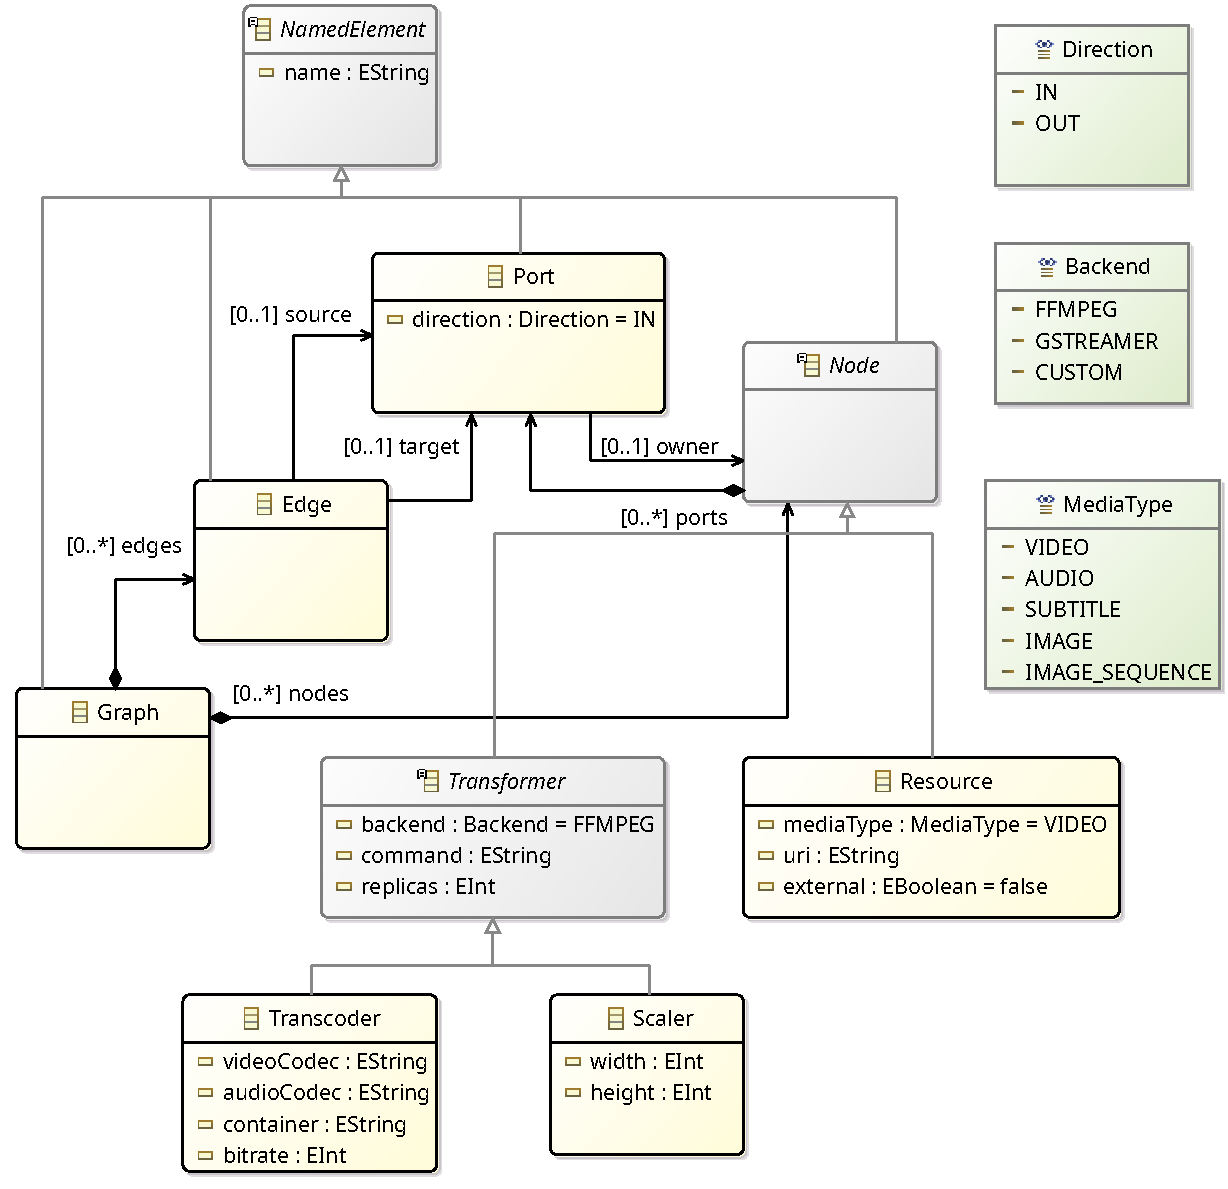
\includegraphics[width=\textwidth]{../figures/mediaflow_class_diagram_cropped.pdf}
\caption{Class diagram metamodel MediaFlow yang menunjukkan hirarki kelas, atribut utama, serta relasi komposisi dan referensi antar elemen domain.}
\label{fig:mediaflow-metamodel-class-diagram}
\end{figure}

Definisi tekstual lengkap metamodel dalam format Emfatic ditunjukkan pada Listing~\ref{lst:mediaflow-emf}. Listing tersebut menjadi acuan formal yang konsisten dengan elemen pada Gambar~\ref{fig:mediaflow-metamodel-class-diagram}.

\begin{lstlisting}[
  language=emfatic,
  caption={Definisi metamodel MediaFlow dalam format Emfatic (\texttt{mediaflow.emf})},
  label={lst:mediaflow-emf},
  basicstyle=\ttfamily\scriptsize
]
@namespace(uri="mediaflow", prefix="mediaflow")
package mediaflow;

enum MediaType {
  VIDEO = 1;
  AUDIO = 2;
  SUBTITLE = 3;
  IMAGE = 4;
  IMAGE_SEQUENCE = 5;
}

enum Backend {
  FFMPEG;
  GSTREAMER;
  CUSTOM;
}

enum Direction {
  IN;
  OUT;
}

abstract class NamedElement {
  attr String name;
}

class Graph extends NamedElement {
  val Node[*] nodes;
  val Edge[*] edges;
}

abstract class Node extends NamedElement {
  val Port[*] ports;
}

class Resource extends Node {
  attr MediaType mediaType;
  attr String uri;
  attr boolean external;
}

abstract class Transformer extends Node {
  attr Backend backend;
  attr String command;
  attr int replicas;
}

class Scaler extends Transformer {
  attr int width;
  attr int height;
}

class Transcoder extends Transformer {
  attr String videoCodec;
  attr String audioCodec;
  attr String container;
  attr int bitrate;
}

class Port extends NamedElement {
  attr Direction direction;
  ref Node owner;
}

class Edge extends NamedElement {
  ref Port source;
  ref Port target;
}
\end{lstlisting}

\section{Model-Model MediaFlow}
\label{sec:model-mediaflow}

Bagian ini menunjukkan dua \textit{instance model} yang \textit{conform} terhadap metamodel pada Section~\ref{sec:metamodel-mediaflow}. Keduanya sama-sama bertipe akar \texttt{mediaflow:Graph}, menggunakan elemen \texttt{nodes} dan \texttt{edges}, serta merealisasikan referensi \texttt{Port.owner}, \texttt{Edge.source}, dan \texttt{Edge.target} sesuai struktur kelas pada metamodel.

\subsection{Model 1: Pipeline Sederhana (\texttt{flow1.model})}

\texttt{flow1.model} memodelkan alur linear: satu \texttt{Resource} input, satu \texttt{Scaler}, dan satu \texttt{Resource} output. Untuk keterbacaan, struktur model berikut ditulis dalam bentuk YAML sebagai representasi konseptual dari instance model yang sama.

\begin{lstlisting}[
  language=yaml,
  caption={Struktur model \texttt{flow1.model} dalam bentuk YAML},
  label={lst:flow1-yaml},
  basicstyle=\ttfamily\scriptsize
]
graph: flow1
nodes:
  - type: Resource
    name: input_video
    external: true
    ports:
      - name: input_video_out
        direction: OUT
  - type: Scaler
    name: scaler_720
    command: scale=1080:720
    replicas: 1
    width: 1080
    height: 720
    ports:
      - name: scaler_720_video_in
        direction: IN
      - name: scaler_720_video_out
        direction: OUT
  - type: Resource
    name: output_video
    external: true
    ports:
      - name: output_video_in
        direction: IN
edges:
  - name: edge_input_video_to_scaler_720
    source: input_video_out
    target: scaler_720_video_in
  - name: edge_scaler_720_to_output_video
    source: scaler_720_video_out
    target: output_video_in
\end{lstlisting}

Listing~\ref{lst:flow1-yaml} memperlihatkan keterkaitan langsung ke metamodel: elemen \texttt{Resource} dan \texttt{Scaler} adalah instansiasi kelas konkret turunan \texttt{Node}; daftar \texttt{ports} merealisasikan relasi kontainmen \texttt{Node.ports}; daftar \texttt{edges} merealisasikan \texttt{Graph.edges}; dan pasangan koneksi \texttt{source}-\texttt{target} merealisasikan referensi \texttt{Edge} ke \texttt{Port}.

\subsection{Model 2: Pipeline Bercabang Multi-Output (\texttt{flow2.model})}

\texttt{flow2.model} memperluas skenario dengan satu node skala 1080p yang bercabang ke dua \texttt{Transcoder} berbeda (H264 dan VP9), lalu berakhir pada dua \texttt{Resource} output. Representasi YAML berikut memperlihatkan struktur yang sama dalam format yang lebih ringkas untuk dokumentasi.

\begin{lstlisting}[
  language=yaml,
  caption={Struktur model \texttt{flow2.model} dalam bentuk YAML},
  label={lst:flow2-yaml},
  basicstyle=\ttfamily\scriptsize
]
graph: flow2
nodes:
  - type: Resource
    name: input_master
    mediaType: VIDEO
    external: true
    ports:
      - name: input_master_out
        direction: OUT
  - type: Scaler
    name: scaler_1080
    backend: FFMPEG
    command: scale=1920:1080
    replicas: 1
    width: 1920
    height: 1080
    ports:
      - name: scaler_1080_in
        direction: IN
      - name: scaler_1080_out_h264
        direction: OUT
      - name: scaler_1080_out_vp9
        direction: OUT
  - type: Transcoder
    name: transcoder_h264
    backend: FFMPEG
    videoCodec: h264
    audioCodec: aac
    container: mp4
    bitrate: 4000
    ports:
      - name: transcoder_h264_in
        direction: IN
      - name: transcoder_h264_out
        direction: OUT
  - type: Transcoder
    name: transcoder_vp9
    backend: GSTREAMER
    videoCodec: vp9
    audioCodec: opus
    container: webm
    bitrate: 2500
    ports:
      - name: transcoder_vp9_in
        direction: IN
      - name: transcoder_vp9_out
        direction: OUT
  - type: Resource
    name: output_mp4
    mediaType: VIDEO
    external: true
    ports:
      - name: output_mp4_in
        direction: IN
  - type: Resource
    name: output_webm
    mediaType: VIDEO
    external: true
    ports:
      - name: output_webm_in
        direction: IN
edges:
  - name: edge_input_to_scaler
    source: input_master_out
    target: scaler_1080_in
  - name: edge_scaler_to_h264
    source: scaler_1080_out_h264
    target: transcoder_h264_in
  - name: edge_scaler_to_vp9
    source: scaler_1080_out_vp9
    target: transcoder_vp9_in
  - name: edge_h264_to_output
    source: transcoder_h264_out
    target: output_mp4_in
  - name: edge_vp9_to_output
    source: transcoder_vp9_out
    target: output_webm_in
\end{lstlisting}

Jika dibandingkan dengan model pertama pada Listing~\ref{lst:flow1-yaml}, model kedua pada Listing~\ref{lst:flow2-yaml} memanfaatkan lebih banyak atribut metamodel: \texttt{backend} (enum \texttt{Backend}), \texttt{mediaType} (enum \texttt{MediaType}), serta atribut spesifik \texttt{Transcoder} seperti \texttt{videoCodec}, \texttt{audioCodec}, \texttt{container}, dan \texttt{bitrate}. Perbandingan ini menegaskan bahwa metamodel yang sama dapat dipakai untuk variasi pipeline sederhana maupun bercabang kompleks.

\section{Representasi Tekstual}
\label{sec:representasi-tekstual}

Setelah model dijelaskan dalam bentuk struktur YAML, bagian ini menunjukkan representasi tekstual berbasis DSL (\textit{Domain-Specific Language}) agar model lebih ringkas dan mudah dibaca manusia. DSL ini tetap \textit{conform} terhadap metamodel yang sama: \texttt{graph} merepresentasikan \texttt{Graph}, deklarasi \texttt{resource}/\texttt{scaler}/\texttt{transcoder} merepresentasikan turunan \texttt{Node}, blok \texttt{port} merepresentasikan \texttt{Port}, dan pernyataan \texttt{edge} merepresentasikan \texttt{Edge}.

\subsection{Sketsa Sintaks DSL}

\begin{lstlisting}[
  language=mediaflow,
  caption={Sketsa sintaks DSL MediaFlow},
  label={lst:mediaflow-dsl-syntax},
  basicstyle=\ttfamily\scriptsize
]
graph <nama_graph> {
  resource <nama_node> [mediaType=<MEDIA_TYPE>] uri="<URI>" external=<true|false> {
    port <nama_port> <IN|OUT>
  }

  scaler <nama_node> backend=<BACKEND> command="<cmd>" replicas=<n> width=<w> height=<h> {
    port <nama_port> <IN|OUT>
  }

  transcoder <nama_node> backend=<BACKEND> command="<cmd>" replicas=<n>
             videoCodec="<v>" audioCodec="<a>" container="<c>" bitrate=<b> {
    port <nama_port> <IN|OUT>
  }

  edge <nama_edge> from <source_port> to <target_port>
}
\end{lstlisting}

\label{subsec:dsl-syntax}
\noindent Listing~\ref{lst:mediaflow-dsl-syntax} mendefinisikan bentuk umum DSL yang dipakai untuk menuliskan model instance secara ringkas namun tetap sejalan dengan struktur metamodel.

\subsection{DSL untuk \texttt{flow1.model}}

\begin{lstlisting}[
  language=mediaflow,
  caption={Representasi DSL untuk model \texttt{flow1.model}},
  label={lst:flow1-dsl},
  basicstyle=\ttfamily\scriptsize
]
graph flow1 {
  resource input_video uri="file:///home/user/alfa/mediaflow/input.mp4" external=true {
    port input_video_out OUT
  }

  scaler scaler_720 backend=FFMPEG command="scale=1080:720" replicas=1 width=1080 height=720 {
    port scaler_720_video_in IN
    port scaler_720_video_out OUT
  }

  resource output_video uri="file:///home/user/alfa/mediaflow/output.mp4" external=true {
    port output_video_in IN
  }

  edge edge_input_video_to_scaler_720 from input_video_out to scaler_720_video_in
  edge edge_scaler_720_to_output_video from scaler_720_video_out to output_video_in
}
\end{lstlisting}

Listing~\ref{lst:flow1-dsl} memperlihatkan bentuk linear dari pipeline sederhana: satu aliran masuk, satu proses transformasi, dan satu keluaran. Secara struktural, model ini identik dengan instance pada Section~\ref{sec:model-mediaflow}, hanya berbeda notasi.

\subsection{DSL untuk \texttt{flow2.model}}

\begin{lstlisting}[
  language=mediaflow,
  caption={Representasi DSL untuk model \texttt{flow2.model}},
  label={lst:flow2-dsl},
  basicstyle=\ttfamily\scriptsize
]
graph flow2 {
  resource input_master mediaType=VIDEO uri="file:///home/user/alfa/mediaflow/master.mov" external=true {
    port input_master_out OUT
  }

  scaler scaler_1080 backend=FFMPEG command="scale=1920:1080" replicas=1 width=1920 height=1080 {
    port scaler_1080_in IN
    port scaler_1080_out_h264 OUT
    port scaler_1080_out_vp9 OUT
  }

  transcoder transcoder_h264 backend=FFMPEG command="ffmpeg -c:v libx264 -c:a aac" replicas=1
             videoCodec="h264" audioCodec="aac" container="mp4" bitrate=4000 {
    port transcoder_h264_in IN
    port transcoder_h264_out OUT
  }

  transcoder transcoder_vp9 backend=GSTREAMER command="vp9enc bitrate=2500 ! webmmux" replicas=2
             videoCodec="vp9" audioCodec="opus" container="webm" bitrate=2500 {
    port transcoder_vp9_in IN
    port transcoder_vp9_out OUT
  }

  resource output_mp4 mediaType=VIDEO uri="file:///home/user/alfa/mediaflow/output-1080p.mp4" external=true {
    port output_mp4_in IN
  }

  resource output_webm mediaType=VIDEO uri="file:///home/user/alfa/mediaflow/output-1080p.webm" external=true {
    port output_webm_in IN
  }

  edge edge_input_to_scaler from input_master_out to scaler_1080_in
  edge edge_scaler_to_h264 from scaler_1080_out_h264 to transcoder_h264_in
  edge edge_scaler_to_vp9 from scaler_1080_out_vp9 to transcoder_vp9_in
  edge edge_h264_to_output from transcoder_h264_out to output_mp4_in
  edge edge_vp9_to_output from transcoder_vp9_out to output_webm_in
}
\end{lstlisting}

Listing~\ref{lst:flow2-dsl} menegaskan bahwa DSL yang sama dapat mengekspresikan topologi bercabang, multi-transformer, dan multi-output tanpa perubahan pada metamodel. Dengan demikian, representasi tekstual ini cocok untuk kebutuhan authoring model, review perubahan, dan integrasi ke alur \textit{model-to-text transformation}.

\section{Representasi Visual}
\label{sec:representasi-visual}

Representasi visual melengkapi representasi YAML (Listing~\ref{lst:flow1-yaml} dan Listing~\ref{lst:flow2-yaml}) serta DSL (Listing~\ref{lst:flow1-dsl} dan Listing~\ref{lst:flow2-dsl}) dengan menampilkan topologi aliran secara langsung. Pada bentuk visual, setiap kotak merepresentasikan instans \texttt{Node}, port ditampilkan sebagai titik koneksi, dan panah merepresentasikan \texttt{Edge}.

\subsection{Visualisasi Pipeline Sederhana (\texttt{flow1.model})}

\begin{figure}[htbp]
\centering
\scalebox{0.7}{
\begin{tikzpicture}[
  node distance=22mm,
  >=Latex,
  flow/.style={draw, rounded corners, minimum width=3.6cm, minimum height=1.0cm, align=center, fill=blue!8},
  proc/.style={draw, rounded corners, minimum width=3.9cm, minimum height=1.0cm, align=center, fill=green!10},
  arr/.style={->, thick}
]
  \node[flow] (in) {\textbf{Resource}\\input\_video};
  \node[proc, right=of in] (scaler) {\textbf{Scaler}\\scaler\_720};
  \node[flow, right=of scaler] (out) {\textbf{Resource}\\output\_video};

  \draw[arr] (in) -- node[above, font=\scriptsize, yshift=15pt]{input\_video\_out $\rightarrow$ scaler\_720\_video\_in} (scaler);
  \draw[arr] (scaler) -- node[above, font=\scriptsize, yshift=15pt]{scaler\_720\_video\_out $\rightarrow$ output\_video\_in} (out);
\end{tikzpicture}
}
\caption{Representasi visual model \texttt{flow1.model}: alur linear Resource $\rightarrow$ Scaler $\rightarrow$ Resource.}
\label{fig:flow1-visual}
\end{figure}

Gambar~\ref{fig:flow1-visual} memperlihatkan topologi linear dengan dua edge. Ini konsisten dengan metamodel: tiga instans \texttt{Node} terhubung melalui pasangan port sumber-target yang valid.

\subsection{Visualisasi Pipeline Bercabang (\texttt{flow2.model})}

\begin{figure}[htbp]
\centering
\scalebox{0.69}{
\begin{tikzpicture}[
  node distance=18mm and 18mm,
  >=Latex,
  res/.style={draw, rounded corners, minimum width=3.2cm, minimum height=0.95cm, align=center, fill=blue!8},
  scl/.style={draw, rounded corners, minimum width=3.4cm, minimum height=0.95cm, align=center, fill=green!10},
  trn/.style={draw, rounded corners, minimum width=3.6cm, minimum height=0.95cm, align=center, fill=orange!14},
  arr/.style={->, thick}
]
  \node[res] (input) {\textbf{Resource}\\input\_master};
  \node[scl, right=of input] (scaler1080) {\textbf{Scaler}\\scaler\_1080};
  \node[trn, right=of scaler1080, yshift=10mm] (h264) {\textbf{Transcoder}\\transcoder\_h264};
  \node[trn, right=of scaler1080, yshift=-10mm] (vp9) {\textbf{Transcoder}\\transcoder\_vp9};
  \node[res, right=of h264] (outmp4) {\textbf{Resource}\\output\_mp4};
  \node[res, right=of vp9] (outwebm) {\textbf{Resource}\\output\_webm};

  \draw[arr] (input) -- node[above, font=\scriptsize, yshift=15pt]{input\_master\_out} (scaler1080);

  \draw[arr] (scaler1080) -- node[above, font=\scriptsize, xshift=-25pt]{scaler\_1080\_out\_h264} (h264);
  \draw[arr] (scaler1080) -- node[below, font=\scriptsize, xshift=-25pt]{scaler\_1080\_out\_vp9} (vp9);

  \draw[arr] (h264) -- node[above, font=\scriptsize, yshift=15pt]{transcoder\_h264\_out} (outmp4);
  \draw[arr] (vp9) -- node[below, font=\scriptsize, yshift=-15pt]{transcoder\_vp9\_out} (outwebm);
\end{tikzpicture}
}
\caption{Representasi visual model \texttt{flow2.model}: topologi bercabang dari satu scaler ke dua transcoder dan dua output.}
\label{fig:flow2-visual}
\end{figure}

Gambar~\ref{fig:flow2-visual} menunjukkan bahwa metamodel yang sama mampu merepresentasikan pola \textit{fan-out} (satu sumber ke banyak cabang). Variasi ini mempertegas fleksibilitas metamodel dalam menangani pipeline linear maupun bercabang tanpa mengubah struktur abstrak.

\section{Ringkasan}

Bab ini menegaskan bahwa \textit{Model-Driven Software Engineering} (MDSE) memindahkan fokus pengembangan dari implementasi langsung ke rekayasa berbasis model. Konsep inti seperti metamodel, model, instance, \textit{abstract syntax}, \textit{concrete syntax}, transformasi M2M/M2T, dan validasi membentuk satu alur yang saling terhubung. Dengan pendekatan ini, struktur domain dapat didefinisikan secara formal, kualitas model dapat dicek lebih awal, dan proses menghasilkan artefak implementasi menjadi lebih konsisten serta terkontrol.

Melalui studi kasus MediaFlow, bab ini menunjukkan bagaimana satu metamodel dapat mendukung berbagai model pipeline, baik linear maupun bercabang, lalu direpresentasikan dalam bentuk tekstual (YAML/DSL) dan visual (diagram). Analogi SVO lintas bahasa juga memperjelas bahwa makna abstrak dapat dipertahankan meskipun bentuk konkret berbeda. Secara praktis, pendekatan MDSE membantu tim mengelola kompleksitas, mengurangi inkonsistensi, dan mempercepat adaptasi perubahan kebutuhan sistem melalui perubahan di level model.
